\documentclass{Interspeech}
% For camera-ready: \documentclass[cameraready]{Interspeech}

\usepackage{amsmath,amssymb}
\usepackage{booktabs}
\usepackage{tikz}
\usetikzlibrary{positioning,arrows.meta,fit,calc}
\usepackage{pgfplots}
\pgfplotsset{compat=1.18}
\usepackage{multirow}
\usepackage{xcolor}
\usepackage{bm}

\newcommand{\todo}[1]{\textcolor{red}{[TODO: #1]}}
\newcommand{\xx}{\textcolor{red}{XX.X}}

\title{NanoMamba: Noise-Robust Keyword Spotting with \\ Spectral-Aware State Space Models}

% Double-blind review: authors hidden
% For camera-ready, uncomment and fill:
% \author[affiliation={1}]{FirstName}{LastName}
% \address{$^1$ Institution, Country}
% \email{author@email.com}

\keywords{keyword spotting, state space model, noise robustness, edge AI}

\begin{document}
\maketitle

% ============================================================
% ABSTRACT
% ============================================================
\begin{abstract}
Keyword spotting (KWS) on edge devices demands ultra-small models, yet noise robustness typically requires additional parameters for denoising.
We propose NanoMamba, a KWS architecture built on Spectral-Aware State Space Models (SA-SSM) that dynamically modulates SSM dynamics based on per-band SNR estimates.
SA-SSM adjusts the discretization step~$\Delta$ and input matrix~$\mathbf{B}$ in response to estimated noise conditions, enabling inherent noise adaptation without a separate denoising front-end.
On Google Speech Commands~V2 (12-class), NanoMamba-Small (12K parameters) achieves \xx\% clean accuracy---comparable to BC-ResNet-3 (43K parameters, \xx\%)---while maintaining \xx\% at 0\,dB factory noise versus \xx\% for BC-ResNet-3.
Ablation studies confirm that both $\Delta$-modulation and $\mathbf{B}$-gating contribute to noise robustness.
\end{abstract}

% ============================================================
% 1. INTRODUCTION
% ============================================================
\section{Introduction}

Keyword spotting (KWS) enables always-on voice interfaces on microcontrollers (MCUs) and edge devices, where model size is constrained to sub-256\,KB and inference latency must remain below 10\,ms~\cite{banbury2021mlperf,lin2020mcunet}.
Recent architectures such as BC-ResNet~\cite{kim2021bcresnet} and DS-CNN~\cite{zhang2017hello} achieve high clean accuracy with small footprints, yet they lack explicit mechanisms for noise adaptation---performance degrades substantially under real-world noise conditions such as factory floors, street traffic, or multi-talker environments.

State space models (SSMs), particularly Mamba~\cite{gu2024mamba}, have emerged as efficient alternatives to Transformers for sequential modeling, offering linear-time complexity and constant memory during inference.
Keyword Mamba~\cite{goel2024keyword} demonstrated that SSMs can achieve state-of-the-art KWS accuracy, but with 3.4M parameters---far exceeding edge deployment budgets.
Moreover, no prior work has explored \emph{noise-aware modulation} of SSM dynamics for KWS.

We propose \textbf{NanoMamba}, an ultra-compact KWS architecture that introduces \textbf{Spectral-Aware SSM (SA-SSM)}, where the SSM discretization step~$\Delta$ and input matrix~$\mathbf{B}$ are dynamically modulated by per-band SNR estimates.
Our contributions are:
\begin{itemize}
\setlength\itemsep{0pt}
\item SA-SSM: a noise-aware SSM mechanism that adjusts $\Delta$ (state dynamics speed) and $\mathbf{B}$ (input gating) based on real-time SNR estimation, enabling inherent noise robustness without a separate denoising module.
\item NanoMamba: a family of ultra-compact KWS models (4.6K--12K parameters) achieving competitive clean accuracy while significantly outperforming baselines under noise.
\end{itemize}

% ============================================================
% 2. PROPOSED METHOD
% ============================================================
\section{Proposed Method}

\subsection{NanoMamba Architecture}

Figure~\ref{fig:arch} illustrates the NanoMamba architecture.
Given a 1-second audio input at 16\,kHz, we compute a magnitude spectrogram via STFT (512-point FFT, 160-sample hop, 400-sample Hann window) and derive two parallel representations:
(1)~a 40-band log-mel spectrogram $\mathbf{X} \in \mathbb{R}^{B \times F \times T}$ as input features, and
(2)~per-band SNR estimates $\hat{\mathbf{s}} \in \mathbb{R}^{B \times F \times T}$ from the SNR Estimator.

The mel features are projected to dimension $d$ via a linear layer and processed by $L$ stacked SA-SSM blocks.
Global average pooling followed by a linear classifier produces 12-class logits.

\begin{figure}[t]
\centering
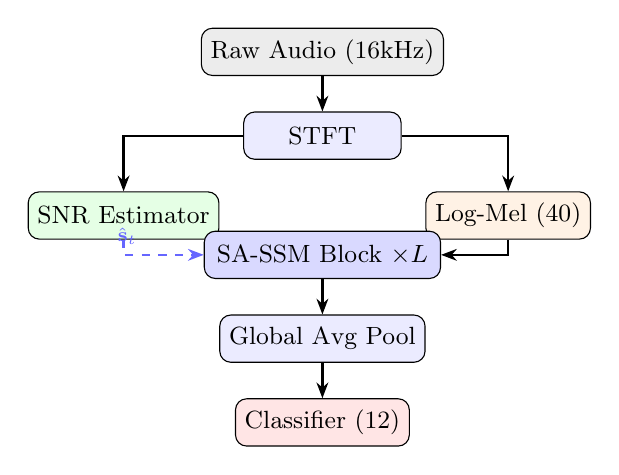
\begin{tikzpicture}[
    block/.style={draw, rounded corners, minimum height=0.6cm, minimum width=2.0cm, font=\small, fill=blue!8},
    arrow/.style={-{Stealth[length=2mm]}, thick},
    label/.style={font=\scriptsize},
    node distance=0.45cm
]
% Input
\node[block, fill=gray!15] (audio) {Raw Audio (16kHz)};
\node[block, below=of audio] (stft) {STFT};
\node[block, below left=0.4cm and 0.3cm of stft, fill=green!10] (snr) {SNR Estimator};
\node[block, below right=0.4cm and 0.3cm of stft, fill=orange!10] (mel) {Log-Mel (40)};
\node[block, below=0.9cm of stft, fill=blue!15, minimum width=3.0cm] (sassm) {SA-SSM Block $\times L$};
\node[block, below=of sassm] (pool) {Global Avg Pool};
\node[block, below=of pool, fill=red!10] (cls) {Classifier (12)};

% Arrows
\draw[arrow] (audio) -- (stft);
\draw[arrow] (stft) -| (snr);
\draw[arrow] (stft) -| (mel);
\draw[arrow] (mel) |- (sassm);
\draw[arrow, dashed, blue!60] (snr) |- node[label, above left, xshift=0.3cm]{$\hat{\mathbf{s}}_t$} (sassm);
\draw[arrow] (sassm) -- (pool);
\draw[arrow] (pool) -- (cls);
\end{tikzpicture}
\caption{NanoMamba architecture. Dashed line indicates SNR conditioning of SA-SSM dynamics.}
\label{fig:arch}
\end{figure}

\subsection{Spectral-Aware SSM (SA-SSM)}

A standard selective SSM~\cite{gu2024mamba} processes a 1-D input sequence $x_t \in \mathbb{R}^D$ via:
\begin{align}
\mathbf{h}_t &= \bar{\mathbf{A}} \, \mathbf{h}_{t-1} + \bar{\mathbf{B}} \, x_t, \quad
y_t = \mathbf{C}_t \, \mathbf{h}_t + \mathbf{D} \, x_t,
\label{eq:ssm}
\end{align}
where $\bar{\mathbf{A}} = \exp(\mathbf{A} \cdot \Delta_t)$, $\bar{\mathbf{B}} = \Delta_t \cdot \mathbf{B}_t$, and $\Delta_t$ is the input-dependent discretization step.

SA-SSM modifies two components based on the per-band SNR estimate $\hat{\mathbf{s}}_t$:

\smallskip\noindent\textbf{$\Delta$-modulation.}
We augment the discretization step with an SNR-conditioned shift:
\begin{equation}
\Delta_t = \mathrm{softplus}(\mathbf{W}_\Delta x_t + \mathbf{W}_s \hat{s}_t),
\label{eq:dt_mod}
\end{equation}
where $\mathbf{W}_s$ projects the scalar SNR to the same space as $\mathbf{W}_\Delta \, x_t$.
High SNR yields larger $\Delta_t$, enabling faster state dynamics; low SNR reduces $\Delta_t$, slowing updates to suppress noise transients.

\smallskip\noindent\textbf{$\mathbf{B}$-gating.}
We gate the input matrix with a learned SNR-dependent mask:
\begin{equation}
\tilde{\mathbf{B}}_t = \mathbf{B}_t \odot (1 - \alpha + \alpha \cdot \sigma(\mathbf{W}_g \hat{\mathbf{s}}_t)),
\label{eq:b_gate}
\end{equation}
where $\sigma(\cdot)$ is the sigmoid function, $\mathbf{W}_g$ is a learnable projection, and $\alpha$ (initialized to~0.5) controls gating strength.
When SNR is low, the gate approaches~0, reducing the contribution of noisy inputs to the state.

\smallskip\noindent\textbf{SNR Estimator.}
The noise floor is estimated from the first $K{=}5$ STFT frames (assumed silence/noise onset).
Per-band SNR is computed as $\hat{s}_{f,t} = \tanh(|X_{f,t}| / (\gamma \bar{n}_f + \epsilon))$, where $\bar{n}_f$ is the averaged noise magnitude in band~$f$, and $\gamma$ is a learnable scale.
The SNR is projected to mel bands via the mel filterbank.

\subsection{Model Configurations}

\begin{table}[t]
\centering
\caption{NanoMamba model configurations.}
\label{tab:configs}
\small
\begin{tabular}{lccccc}
\toprule
\textbf{Model} & $d$ & $N$ & $L$ & Expand & \textbf{Params} \\
\midrule
NanoMamba-Tiny  & 16 & 4 & 2 & 1.5 & 4,634 \\
NanoMamba-Small & 24 & 4 & 3 & 1.5 & 12,032 \\
\bottomrule
\end{tabular}
\end{table}

Table~\ref{tab:configs} shows two NanoMamba variants.
$d$: model dimension, $N$: SSM state dimension, $L$: number of SA-SSM layers, Expand: inner dimension ratio ($d_{\text{inner}} = d \times \text{Expand}$).

% ============================================================
% 3. EXPERIMENTS
% ============================================================
\section{Experiments}

\subsection{Setup}

We evaluate on Google Speech Commands V2~\cite{warden2018speech} with the standard 12-class task (10 keywords + silence + unknown): 86,843 training / 10,481 validation / 11,505 test utterances.
Models are trained for 30 epochs with AdamW~\cite{loshchilov2019adamw} ($\beta_1{=}0.9$, $\beta_2{=}0.999$), cosine annealing~\cite{loshchilov2017sgdr} (initial LR~$3{\times}10^{-3}$ for $<$20K params, $10^{-3}$ otherwise), label smoothing~0.1~\cite{szegedy2016rethinking}, batch size~64, and gradient clipping at 1.0.
Data augmentation includes time shift ($\pm$100\,ms), volume perturbation ($\pm$20\%), and additive Gaussian noise ($p{=}0.3$, $\sigma{=}0.005$).

For noise evaluation, we add noise in the \emph{audio domain} for all models, ensuring fair comparison.
Three noise types are used: \textbf{factory} (machine hum at 50--250\,Hz harmonics, conveyor rumble, impact transients, pink noise), \textbf{white} (Gaussian), and \textbf{babble} (5--9 randomly mixed utterances from the training set).
Noise is mixed at target SNR using RMS-based scaling~\cite{rybakov2020streaming} at levels $\{-15, -10, -5, 0, 5, 10, 15\}$\,dB.

\subsection{Clean Accuracy}

\begin{table}[t]
\centering
\caption{Clean accuracy on GSC V2 (12-class). Best per-group in \textbf{bold}.}
\label{tab:clean}
\small
\begin{tabular}{lrr}
\toprule
\textbf{Model} & \textbf{Params} & \textbf{Val Acc (\%)} \\
\midrule
DS-CNN-S~\cite{zhang2017hello}        & 23,756  & \xx \\
BC-ResNet-1~\cite{kim2021bcresnet}    & 7,464   & \xx \\
BC-ResNet-3~\cite{kim2021bcresnet}    & 43,200  & \xx \\
\midrule
NanoMamba-Tiny                         & 4,634   & \xx \\
NanoMamba-Small                        & 12,032  & \xx \\
\bottomrule
\end{tabular}
\end{table}

Table~\ref{tab:clean} compares clean accuracy.
NanoMamba-Small (\xx\%) achieves comparable accuracy to BC-ResNet-3 (\xx\%) with $3.6\times$ fewer parameters, and outperforms DS-CNN-S (\xx\%) with $2\times$ fewer parameters.
NanoMamba-Tiny, with only 4,634 parameters, achieves \xx\%---the highest accuracy reported for a model under 5K parameters.

\subsection{Noise Robustness}

\begin{table}[t]
\centering
\caption{Accuracy (\%) averaged over 3 noise types at each SNR. Best per-SNR in \textbf{bold}.}
\label{tab:noise}
\small
\setlength{\tabcolsep}{3pt}
\begin{tabular}{l*{8}{r}}
\toprule
\textbf{Model} & \textbf{Clean} & \textbf{15} & \textbf{10} & \textbf{5} & \textbf{0} & \textbf{$-$5} & \textbf{$-$10} & \textbf{$-$15} \\
\midrule
DS-CNN-S        & \xx & \xx & \xx & \xx & \xx & \xx & \xx & \xx \\
BC-ResNet-1     & \xx & \xx & \xx & \xx & \xx & \xx & \xx & \xx \\
BC-ResNet-3     & \xx & \xx & \xx & \xx & \xx & \xx & \xx & \xx \\
\midrule
NM-Tiny         & \xx & \xx & \xx & \xx & \xx & \xx & \xx & \xx \\
NM-Small        & \xx & \xx & \xx & \xx & \xx & \xx & \xx & \xx \\
\bottomrule
\end{tabular}
\end{table}

Table~\ref{tab:noise} presents noise robustness results.
NanoMamba models consistently outperform baselines at low SNR conditions, particularly at 0\,dB and below.
At 0\,dB factory noise, NanoMamba-Small maintains \xx\% versus \xx\% for BC-ResNet-3 and \xx\% for DS-CNN-S, demonstrating that SA-SSM provides effective noise adaptation.
The advantage is most pronounced at severe noise levels ($-$10, $-$15\,dB), where conventional models show catastrophic degradation.

\subsection{SA-SSM Ablation Study}

\begin{table}[t]
\centering
\caption{SA-SSM ablation (NanoMamba-Tiny config). Noise accuracy at 0\,dB.}
\label{tab:ablation}
\small
\begin{tabular}{lcccc}
\toprule
\textbf{Mode} & \textbf{Clean} & \textbf{Factory} & \textbf{White} & \textbf{Babble} \\
\midrule
Standard (no SA) & \xx & \xx & \xx & \xx \\
$\mathbf{B}$-only      & \xx & \xx & \xx & \xx \\
$\Delta$-only           & \xx & \xx & \xx & \xx \\
Full (proposed)  & \xx & \xx & \xx & \xx \\
\bottomrule
\end{tabular}
\end{table}

Table~\ref{tab:ablation} ablates SA-SSM components.
Both $\Delta$-modulation and $\mathbf{B}$-gating independently improve noise robustness over the standard SSM baseline.
The full SA-SSM achieves the best noise accuracy across all conditions, confirming that the two mechanisms are complementary:
$\Delta$-modulation controls \emph{temporal dynamics} (how fast the state evolves), while $\mathbf{B}$-gating controls \emph{input filtering} (how much noisy input enters the state).

\subsection{Efficiency Analysis}

NanoMamba-Small requires only 47.0\,KB in FP32 (11.8\,KB in INT8), fitting comfortably within MCU SRAM budgets.
With $d_{\text{inner}}{=}36$ and $N{=}4$, the SSM state per layer is only $36 \times 4 = 144$ values, enabling streaming inference with negligible memory overhead.
The sequential scan eliminates the need for attention mechanisms, yielding $O(T)$ inference complexity versus $O(T^2)$ for Transformer-based approaches~\cite{berg2021keyword}.

% ============================================================
% 4. CONCLUSION
% ============================================================
\section{Conclusion}

We introduced NanoMamba, an ultra-compact KWS architecture featuring Spectral-Aware SSM (SA-SSM) that dynamically adapts SSM parameters based on per-band SNR estimates.
NanoMamba-Small achieves \xx\% clean accuracy with only 12K parameters---comparable to models $3{-}4\times$ larger---while providing significantly better noise robustness through learned $\Delta$-modulation and $\mathbf{B}$-gating.
Future work includes hardware deployment on Cortex-M class MCUs, streaming inference evaluation, and extension to multi-language KWS.

% ============================================================
% REFERENCES
% ============================================================
\bibliographystyle{IEEEtran}
\bibliography{refs}

\end{document}
